\documentclass[a4paper, 12pt, oneside]{book}
\usepackage{amssymb}

\usepackage{xspace}
\usepackage{tikz}
\usepackage{subcaption}

\usetikzlibrary{automata,arrows,positioning,calc}
\usepackage{tabls}
\usepackage{float}
\usepackage[newitem,newenum,neverdecrease]{paralist}
\usepackage{amsmath,amssymb,amsfonts,mathrsfs,latexsym,stmaryrd}
\usepackage{mathtools}
\usepackage{amsthm}
\usepackage{ifpdf}
\usepackage{cases}
\usepackage{ragged2e} 	% https://tex.stackexchange.com/questions/89680/how-can-one-set-full-justification-within-left-justified-raggedright-text
\usepackage{breakcites} % https://tex.stackexchange.com/questions/2773/how-do-i-make-latex-push-long-citations-to-a-new-line
\usepackage{hyperref}	% http://tex.stackexchange.com/questions/73862/how-can-i-make-a-clickable-table-of-contents
\usepackage{fancyhdr}	% https://www.sharelatex.com/blog/2013/08/06/thesis-series-pt2.htmlhttps://www.overleaf.com/project/600b9de46cd176f41d036aed
\usepackage{titlesec} 	% http://tex.stackexchange.com/questions/11444/how-to-format-the-chapter-heading
\usepackage[T1]{fontenc}
\usepackage[utf8]{inputenc}
%\usepackage{setspace}
\usepackage{xcolor}
\usepackage{geometry}
\usepackage{listings}
\usepackage[listings]{tcolorbox}
\newtcblisting[auto counter]{lists}[1][0]{ 
    colframe=black, colback=white, listing only, 
    listing options={basicstyle=\ttfamily,language=prolog} 
}
\usepackage{layout}		% http://tex.stackexchange.com/questions/50258/margins-of-book-class

%%% Formattazione del header del Capitolo
\titleformat
{\chapter} % command
[display] % shape
{\bfseries\Huge\itshape} % format
{\flushright \color{black!45}{\Large Chapter \thechapter}} % label
{0.5ex} % sep
{
    \rule{\textwidth}{3pt}
    \vspace{1ex}
    \centering
} % before-code
[
\vspace{-0.5ex}%
\rule{\textwidth}{3pt}
] % after-code
%%% end

%%% Formattazione dei hyper riferimenti (hyperref)
% hyperref setup -- http://tex.stackexchange.com/questions/73862/how-can-i-make-a-clickable-table-of-contents
\definecolor{Aqua}{rgb}{0,0.45,0.45}
\definecolor{Gold}{rgb}{0.55,0.55,0}
\hypersetup{
    % bookmarks=true,         % show bookmarks bar?
    unicode=false,          % non-Latin characters in Acrobat’s bookmarks
    pdftoolbar=true,        % show Acrobat’s toolbar?
    pdfmenubar=true,        % show Acrobat’s menu?
    pdffitwindow=false,     % window fit to page when opened
    pdfstartview={FitH},    % fits the width of the page to the window
    pdftitle={Implementation of a Tableau-Based Satisfiability Checker for the Logic HS3},    % title
    pdfauthor={Gianluca Maselli},     % author
    pdfsubject={Interval Temporal Logic},   % subject of the document
    pdfcreator={Stan Ionel Eduard},   % creator of the document
    pdfproducer={Stan Ionel Eduard}, % producer of the document
    pdfkeywords={Modal and Temporal Logic, (Un)Decidibility, Complexity, SAT checker}, % list of keywords
    linktocpage=false,		% number hyperref'd =true, false otherwise
    pdfnewwindow=true,      % links in new PDF window
    colorlinks=true,       % false: boxed links; true: colored links
    linkcolor=Aqua,          % color of internal links (change box color with linkbordercolor)
    citecolor=magenta,        % color of links to bibliography
    filecolor=green,      % color of file links
    urlcolor=Gold           % color of external links
}
%%% end

% https://tex.stackexchange.com/questions/95488/list-of-figures-and-page-numbering
\makeatletter
\newcommand{\emptypage}[1]{%
  \cleardoublepage
  \begingroup
  \let\ps@plain\ps@empty
  \pagestyle{empty}
  #1
  \cleardoublepage}
\makeatletter

% base line strech (default 1.0) -- interlinea
\renewcommand{\baselinestretch}{1.2}

\begin{document}
%%% Nuova geometria per la pagina del titolo
% visto che la classe del documento è book, le pagine pari e dispari avranno geometrie diverse,
% mentre quella del titolo deve essere unica!
\newgeometry{
  top=2cm,
  bottom=2.5cm,
  left=2.5cm,
  right=2.5cm,
  headsep=25pt,
  headheight=14.5pt
}

%%% Pagina del titolo
\begin{titlepage}
    \topskip0pt
	%\vspace*{\fill}
	\centering
	\vspace*{1mm}
	
\includegraphics[width= 4cm ]{figures/Logo.png}\\
	\vspace*{1cm}
	\huge \textbf{\textsc{Sapienza Università di Roma}}\\
	\Large \textsc{Master: Artificial Intelligence and Robotics}
	\topskip0pt
	%\vspace*{\fill}
	\centering
	\vspace*{5mm}
	\vspace*{1cm}
	
	\vspace*{1.5cm}
	\hrule width \hsize \kern 1mm \hrule width \hsize height 2pt
	\vspace*{10mm}
	\Huge \emph{\textbf{Coppelia Scene: Omnidirectional MultiRotor UAV}}
	\vspace*{10mm}
	\hrule width \hsize height 2pt
	\vspace*{1mm}
	\hrule width \hsize \kern 1mm
	
	\vspace*{10mm}
    \begin{center}
        \Large \textbf{Akshay Dhonthi Ramesh Babu - 1887502}\\
        \Large \textbf{Fabian Humberto Fonseca Aponte - 1886565}\\
		\Large \textbf{David Esteban Imbajoa Ruiz - 1922212}
		\end{center}
	
	\vspace*{20mm}
	\Large \textsc{Academic Year $2020-2021$}
	
\end{titlepage}
% \restoregeometry
\newgeometry{
  top=3.5cm,
  bottom=2.5cm,
  left=2.5cm,
  right=2.5cm,
  headsep=25pt,
  headheight=14.5pt
}
\addtocontents{toc}{~\hfill\textbf{Page}\par}	% https://texblog.org/2011/09/09/10-ways-to-customize-tocloflot/
\pagestyle{empty}
\clearpage
\tableofcontents
\thispagestyle{empty}
\addtocontents{toc}{\protect\thispagestyle{empty}}	% http://tex.stackexchange.com/questions/2995/removing-page-number-from-toc

\chapter{Introduction}\label{int}
Since the development of the first manned aircraft, which was one of the great milestones of humanity, ways of improvement and optimization have been sought in order to have progressively greater autonomy and less responsibility on the side of the pilot. This is why after the appearance of vehicles with vertical take-off humanity had pillars to develop drones, from this point there was a chain of developments aimed at reducing the size and increasing the maneuverability of these devices, each one of them carries its own challenges and requirements at the design and control level.\\

This line of research has made considerable progress in recent years and in different branches, depending on the number of actuators, physical arrangement and control. Authors such as Hamandi \cite{hamandi2020survey} have dedicated an effort to study the beginnings of these technologies, their ramifications as well as their possible research sectors. His work has been so detailed that the taxonomic description of drones provided by the author takes into consideration all the factors mentioned above to define specific clusters on the subject, raising concepts such as Fully Actuated Drones (FAD) and Over Actuated Drones (OAD) which take an important part of this project.\\

From this classification, different research topics can be obtained that are broad enough to deserve a line of research by themselves in each of their categories, such as path planning, location, mapping and control theory. Sometimes they have their own peculiarities as the same author expresses in relation to the atomic number of  actuation units (AAU), the number of propellers and all the characteristics with which the performance of a drone can be evaluated.\\

Throughout this ocean of research alternatives it is useful to define a narrow scope in benefit of any project, in the case of the present work it is expected to design a simulation environment in CoppeliaSim with a fully actuated and omni-directional drone from which it can be designed, implemented and evaluate position and attitude control alternatives. With this purpose a scene was built from scratch with a drone that has 3 degrees of freedom in each of its 4 propellers, its dynamics were programmed in the CoppeliaSim script to enable its control in the simulation environment.\\
    
Due to the number of variables to control in the propellers, the modeled drone falls into the category of a quad-rotor over-actuated whose dynamic modeling and control is normally guided by researches such as the ones held by the authors Falconi \cite{falconi2012dynamic} and Ryll \cite{ryll2013first}\cite{ryll2012modeling}, and it is possible to highlight the level of detail achieved by the author \c{S}enkul when designing a control system that explicitly includes the radial and tangential tilt functions in his propellers\cite{csenkul2016system}. However, for the present work and in accordance with the work of Kumar \cite{kumar2017position}, a direct assumption is made that simplifies the model towards a fully actuated quad-rotor from the control experiments presented in this report can be performed.\\

This text is organized as follows: The chapter \ref{bk} of basic knowledge with the considerations of the model used, the mechanical design and the equations that model its control, followed by the chapters \ref{meth} and \ref{impl} with the methodology used during the controller and CAD design, its integration into of the CoppeliaSim scene, the considerations taken into account during the programming of the model and the tuning process of the control gains, the chapter \ref{expe} contains the experiments carried out to evaluate the performance of the obtained model and ends with the chapters \ref{conclu} that contain the results and conclusions respectively.

%%% Fancy header settings, queste impostazioni vanno fatte solo una volta all'inizio del primo capitolo!
\pagestyle{fancy}
\fancyhf{}
\renewcommand{\headrulewidth}{2pt}
\fancyhead[L]{\textbf{\textsf{\nouppercase\thepage}}}
\fancyhead[R]{\textbf{\textsf{\nouppercase\leftmark}}}
\fancyhead[OR]{\textbf{\textsf{\nouppercase\thepage}}}
\fancyhead[OL]{\textbf{\textsf{\nouppercase {\rightmark}}}}
%%% end

\chapter{Basic Knowledge}\label{bk}

This chapter presents the mechanical design associated with the quad-rotor in the section \ref{mech_des}, followed by the design of the model associated with the control of the UAV in the section \ref{model}, both sections have the basic theory considered for the project with the required nomenclature, the taxonomy that characterizes the drone used for the present project.

\section{Mechanical design}\label{mech_des}
The mechanical design taken into account for this project is the one of a quad-rotor, a UAV with four propellers, which with the intention of maintaining a constant or almost constant center of mass have a symmetric distribution with respect to its geometric center. In the same way, with the goal of simplifying the simulation as much as possible, the mechanical design does not take into account the influence of electronic components or motors on their mass or inertia during its operation, however in its conception it does include the joints required to perform the tasks or rotations in the R2 plane see figure \ref{fig:joint_r2}.

\begin{figure}[H]
    \begin{center}
        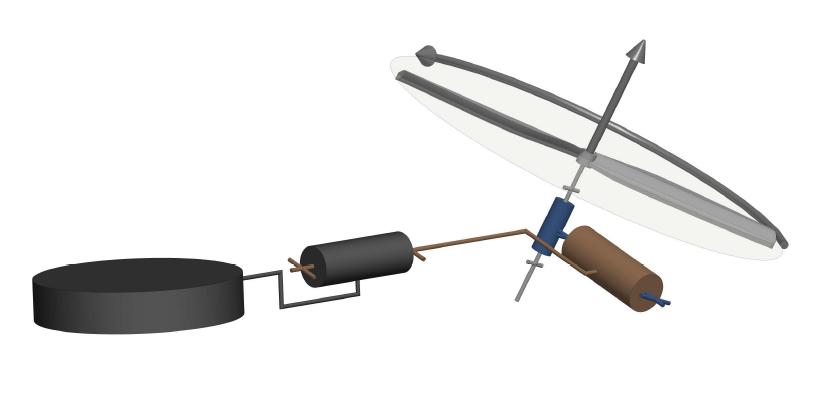
\includegraphics[width=.5\linewidth]{figures/joint_r2.PNG}
        \caption{Single kinematic chain for a propeller with two degrees of freedom \cite{hamandi2020survey}.}
        \label{fig:joint_r2}
    \end{center}
\end{figure}

\subsection{Characterization of the atomic actuation units}
According to the author Hamandi, there are 4 specific parameters to characterize the atomic actuation units (AAU), which must be defined to delimit the scope of the modeling and the influence of the control signals on the behavior of the UAV.

\begin{itemize}
    \item \textbf{Aerodynamic coefficients}, which are constant for the propellers and in the case of this project do not affect the simulation process, the model used or the resulting control loop.
    \item \textbf{Unidirectional or bidirectional thrust}, a parameter that depends directly on the motor whether it is enabled to rotate in both directions or in one direction only, for this project it is assumed that it will be unidirectional.
    \item \textbf{Fixed or actuated propulsion shafts}, defines whether the frame that supports the propellers is a rigid body along with the rest of the structure or has actuated joints, the fixed propeller being the simplest control case. For the present project, we have propellers actuated with two degrees of freedom.
    \item \textbf{Position of the propellers}, is the parameter that defines the spatial location of each of the propellers with respect to the main body of the drone, it is important to define the effect that each one of them has in terms of force and moment and what is the contribution that this means in the movement. In the case of this project, this parameter is constant and does not affect the simulation since the power design of the motors is not being taken into account.
\end{itemize}

\subsection{Properties of the designed system}
From the multiple kinds of UAVs, the one proposed by this project meets the conditions of an over actuated drone due to the fact that more control inputs are required to obtain a trajectory in the space determined by the application. However, again following the recommendations of the author Kumar it is possible to reduce the number of control inputs by mirroring the configuration or orientation of opposing propellers, under these conditions the drone has the characteristics of a Fully Actuated FA and Omni Directional OD drone, and from this classification some properties of the system can be analyzed:


\begin{itemize}
    \item \textbf{Hovering Ability}, is the ability to maintain a constant configuration (position and orientation) even though these possible configurations are only a subset of all transition ones. Since the considered UAV belongs to the omnidirectional category, it can hover with any orientation.
    \item \textbf{Trajectory Tracking Ability}, consists of the ability to track the trajectory of position and orientation in space, giving priority to position tracking in 3D, and allowing access to orientation tracking by modifying the UAV design progressively until it reaches the orientation tracking in 3D.
    \item \textbf{Physical Interaction Ability}, enables the drone to interact with the environment through the exchange of forces, however, since the design of the motors is not being taken into account in this project, nor is any robust control method that handles the change of mass or its center of mass, it is assumed that the UAV used does not have this capacity.
\end{itemize}

\section{Modeling the quad-rotor}\label{model}
From the work carried out by the author Hamandi, there is a general notion of the state of the art in terms of quadrotor designs, that is, UAVs that have 4 AAUs with their different variations, which include fixed propellers, with a tangential tilt design, as well as radial and mixed.

\begin{figure}[H]
\centering
\begin{subfigure}{.49\textwidth}
  \centering
  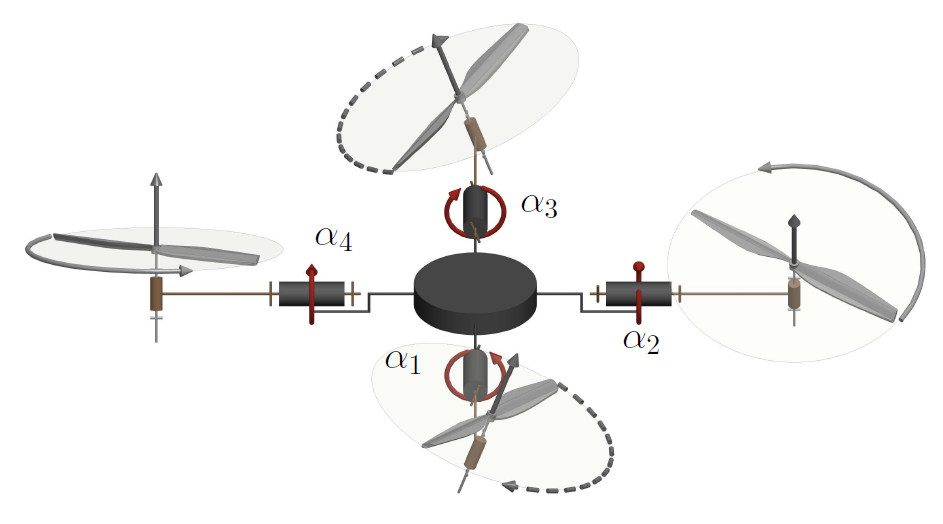
\includegraphics[width=.99\linewidth]{figures/radial_UAV.PNG}
  \caption{Radial tilt design.}
  \label{fig:radial_UAV}
\end{subfigure}
\begin{subfigure}{.49\textwidth}
  \centering
  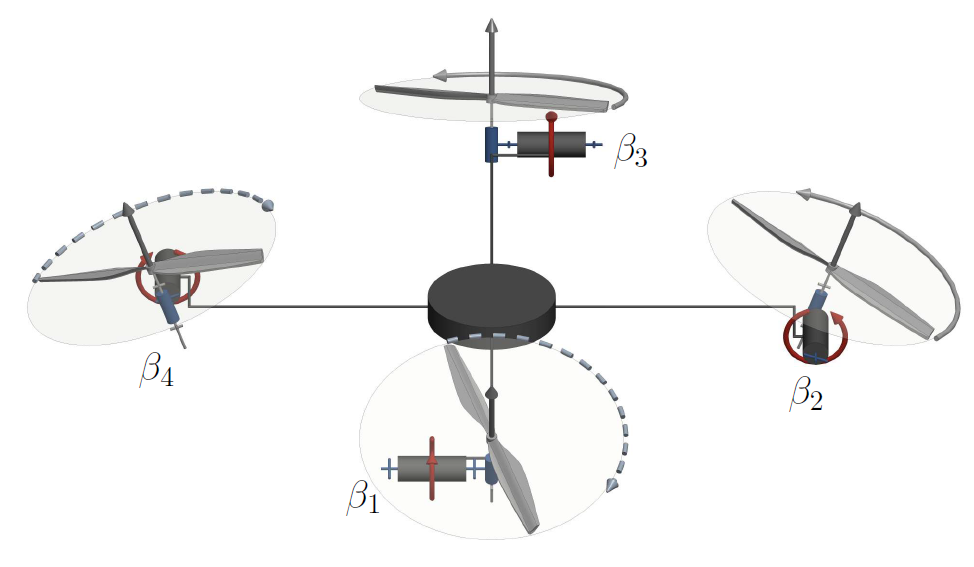
\includegraphics[width=.99\linewidth]{figures/tangential_UAV.PNG}
  \caption{Tangential tilt design.}
  \label{fig:tangential_UAV}
\end{subfigure}
\begin{subfigure}{.49\textwidth}
  \centering
  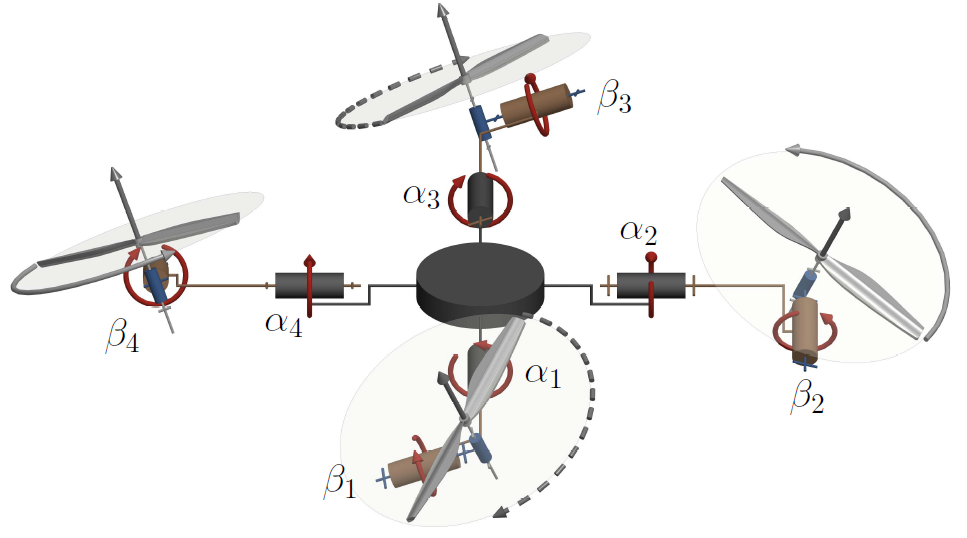
\includegraphics[width=.99\linewidth]{figures/mixed_UAV.PNG}
  \caption{Mixed Tilt Design (Radial and Tangential).}
  \label{fig:mixed_UAV}
\end{subfigure}
\caption{Design alternatives for quadrotor \cite{hamandi2020survey}.}
\label{fig:patch_extraction}
\end{figure}

In this project and with the aim of providing a suitable platform for future developments, it  was designed an UAV that meets the mechanical characteristics in order to have a mixed inclination in $\mathbb{S}^2$ (Figure \ref{fig:mixed_UAV}), using both radial and tangential axes. However, in the scope defined for the implementation of the project, only the degrees of freedom associated with the radial inclination are used (Figure \ref{fig:radial_UAV}), meaning that the design used for the control and fulfillment of the requirements is the UAV with the radial tilting achieving thrust vectoring.

\subsection{Kinematic model}
As is common in all robotic systems, it must be taken into account that the interactions, forces and control signals have an effect in points far from the general center of mass of the system, and in order to properly study their effects these vectors must be transformed to the coordinate system of interest. In the case of the UAV considered for this project, the coordinate axes of the figure \ref{fig:kin_UAV} are assigned, one for the base of the drone, one for each propellant that is repeated in its counterparts and one for the environment.

\begin{figure}[H]
    \begin{center}
        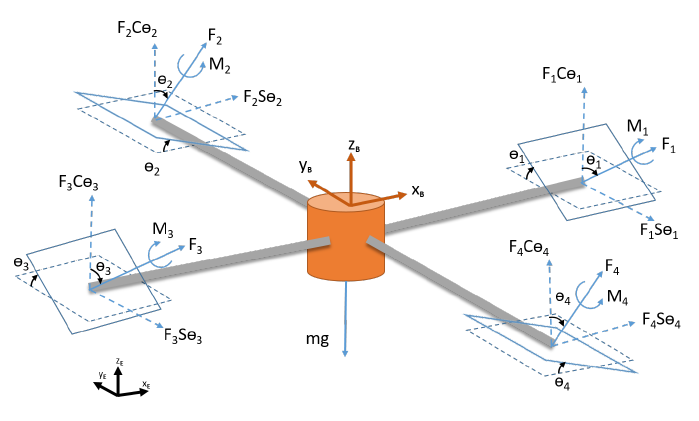
\includegraphics[width=.75\linewidth]{figures/kin_UAV.PNG}
        \caption{Kinematic model for an UAV with radial tilting \cite{kumar2017position}.}
        \label{fig:kin_UAV}
    \end{center}
\end{figure}

In the diagram it can be seen that the assumed design corresponds to the one with the radial inclination enabled, taking the $\theta_i$ values for each of the 4 propellers, modifying the direction of the generated impulse with the equation \ref{eq:rotationBE}.

\begin{equation}
R_{B/E} = 
\begin{bmatrix}
    \cos\psi\cos\theta & \cos\psi\sin\theta\sin\phi-\sin\psi\cos\phi & \cos\psi\sin\theta\cos\phi+\sin\psi\sin\phi\\ 
    \sin\psi\cos\theta & \sin\psi\sin\theta\sin\phi+\cos\psi\cos\phi & \sin\psi\sin\theta\cos\phi-\cos\psi\sin\phi\\ 
    -\sin\theta & \cos\theta\sin\psi & \cos\theta\cos\psi
\end{bmatrix}
\label{eq:rotationBE}
\end{equation}

In a similar way, the acceleration equations associated with the moment equations of the frame of reference of the drone body can be obtained. Using the Newton-Euler method, the equations of motion with respect to the global reference frame can be represented in the equation \ref{eq:motion_world}, in which $m$ is the mass of the UAV, $C_i$ are the drag coefficients and $F_i$ are the forces produced by the propellers according to the equation \ref{eq:propeller_force}.

\begin{equation}
\begin{bmatrix}
\ddot{x}\\ 
\ddot{y}\\ 
\ddot{z}
\end{bmatrix}
=
\frac{R_{B/E}}{m}
\begin{bmatrix}
F_2\sin\theta_2+F_4\sin\theta_4\\ 
-F_1\sin\theta_1-F_3\sin\theta_3\\ 
F_1\cos\theta_1+F_2\cos\theta_2+F_3\cos\theta_3+F_4\cos\theta_4
\end{bmatrix}
-
\begin{bmatrix}
C_1\dot{x}\\ 
C_2\dot{y}\\ 
C_3\dot{z}+g
\end{bmatrix}
\label{eq:motion_world}
\end{equation}

\begin{equation}
F_i=k_fw_i^2
\label{eq:propeller_force}
\end{equation}

The equation for global drone orientation change can be represented in an analogous way, taking into account that $p$ $q$ and $r$ are the roll rate, pitch rate and yaw rate with respect to the reference frame of the drone body.

\begin{equation}
\begin{bmatrix}
\dot{\phi}\\ 
\dot{\theta}\\ 
\dot{\psi}
\end{bmatrix}
=
\begin{bmatrix}
1 & \sin\phi\frac{\sin\theta}{\cos\theta} & \cos\phi\frac{\sin\theta}{\cos\theta} \\ 
0 & \cos\phi & -\sin\phi \\ 
0 & \frac{\sin\phi}{\cos\theta} & \frac{\cos\phi}{\cos\theta}
\end{bmatrix}
\begin{bmatrix}
p\\ 
q\\ 
r
\end{bmatrix}
\label{eq:rotation_world}
\end{equation}

With this model and these equations as a reference, it is possible to proceed with the design of the controller in the chapter \ref{meth} and the implementation of the project in the chapter \ref{impl}.

\chapter{Methodology}\label{meth}
This chapter presents the considerations taken into account by the author Kumar in the design of the quadrotor control as well as the methodology that is expected to be used during the development of the project.

\section{Control design}\label{control}
The design process begins by analyzing the requirements of the drone, which by having the angular velocity of its 4 propellers and the angular position of the radial inclination of the same 4 propellers, it has a total of 8 control inputs for a 6-dimensional workspace: 3 for position and 3 for orientation of the drone body in space.\\

Due to these characteristics and with the intention of simplifying the controller model, it is sought to reduce the number of inputs to 6 by making the UAV Fully Actuated by matching the values of the angular position of the opposite joints according to the equation \ref{eq:match_angle}.

\begin{equation}
\begin{multlined}
\theta_1=\theta_3 \\
\theta_2=\theta_4
\end{multlined}
\label{eq:match_angle}
\end{equation}

With this simplification you can proceed with the design of the control of position an attitude.

\subsection{Position and attitude control}
Defining in a classic way the errors in position and speed with respect to the global coordinate axes, in which the position given by the feedback is compared with the desired position as represented by the \ref{eq:errors} equations.

\begin{equation}
\begin{split}
e=\begin{bmatrix}
e_x\\ 
e_y\\ 
e_z
\end{bmatrix}
=
\begin{bmatrix}
x_{des} - x \\ 
y_{des} - y\\ 
z_{des} - z
\end{bmatrix}\\
\dot{e}=\begin{bmatrix}
\dot{e_x}\\ 
\dot{e_y}\\ 
\dot{e_z}
\end{bmatrix}
=
\begin{bmatrix}
\dot{x_{des}} - \dot{x} \\ 
\dot{y_{des}} - \dot{y}\\ 
\dot{z_{des}} - \dot{z}
\end{bmatrix}
\end{split}
\label{eq:errors}
\end{equation}

It is possible to define a PD control for the calculation of the desired acceleration with respect to the global reference frame using proportional and derivative gains, and take the resulting equation \ref{eq:acc_des} to define the angular velocity required for hovering as well as its change in velocity to generate a motion along the Z-axis in the equations \ref{eq:w} and \ref{eq:dw} respectively.

\begin{equation}
\ddot{r_{des}}=k_{pi}e_i+k_{di}\dot{e_i}=
\begin{bmatrix}
k_{px}e_x\\ 
k_{py}e_y\\ 
k_{pz}e_z
\end{bmatrix}
+
\begin{bmatrix}
k_{dx}\dot{e_x}\\ 
k_{dy}\dot{e_y}\\ 
k_{dz}\dot{e_z}
\end{bmatrix}
;
\forall i \in \left \{ x, y, z \right \}
\label{eq:acc_des}
\end{equation}

\begin{equation}
w_h=\sqrt{\frac{mg}{2k_f(\cos\theta_1+\cos\theta_2)}}
\label{eq:w}
\end{equation}

\begin{equation}
\Delta w_h=\frac{m\ddot{r_z}^{des}}{4k_fw_h(\cos\theta_1+\cos\theta_2)}
\label{eq:dw}
\end{equation}

In order to calculate the desired orientation in the Euler angles, the equation \ref{eq:acc_des} and the angle $\psi$ are used, which are the bases to obtain the equations \ref{eq:phi_des} and \ref{eq:theta_des}, and with these values the errors associated can be calculated by feedback comparison.

\begin{equation}
\phi^{des}=\frac{\ddot{r_x}^{des}\sin\psi^{des}-\ddot{r_y}^des\cos\psi^{des}}{g}
\label{eq:phi_des}
\end{equation}

\begin{equation}
\theta^{des}=\frac{\ddot{r_x}^{des}\cos\psi^{des}-\ddot{r_y}^des\sin\psi^{des}}{g}
\label{eq:theta_des}
\end{equation}

The final design of the control represented in the \ref{eq:full_control} equations, seeks that the rotor 1 and 3 control the position in Y and the roll angle, while the rotors 2 and 4 control the position X and the pitch angle.

\begin{equation}
\begin{split}
\Delta w_\phi=k_{p,\phi}(\phi^{des}-\phi)+k_{d,\phi}(p^{des}-p)\\
\Delta w_\theta=k_{p,\theta}(\theta^{des}-\theta)+k_{d,\theta}(q^{des}-q)\\
\Delta w_\psi=k_{p,\psi}(\psi^{des}-\psi)+k_{d,\psi}(r^{des}-r)\\
\Delta \theta_{T_\phi}=k_{p,\phi_T}(\phi^{des}-\phi)+k_{d,\phi_T}(p^{des}-p)\\
\Delta \theta_{T_\theta}=k_{p,\theta_T}(\theta^{des}-\theta)+k_{d,\theta_T}(q^{des}-q)\\
\Delta \theta_{T_x}=k_{p,x_T}e_x+k_{d,x_T}\dot{e_x}\\
\Delta \theta_{T_y}=k_{p,y_T}e_y+k_{d,y_T}\dot{e_y}
\end{split}
\label{eq:full_control}
\end{equation}

$\Delta w_i, \forall i \in \left \{ \phi, \theta, \psi \right \}$ represents the change in angular velocity needed in the rotors to achieve effective control over orientation, while $\Delta \theta_{T_i}, \forall i \in \left \{ x, y, \phi, \theta \right \}$ represents the change in pitch required in the rotors to achieve pose (position and orientation) control. A final representation of the control inputs can be obtained as a linear combination of the equations \ref{eq:phi_des}, \ref{eq:theta_des} and \ref{eq:full_control} resulting in the following equation:

\begin{equation}
\begin{bmatrix}
w_1^{des}\\ 
w_2^{des}\\ 
w_3^{des}\\ 
w_4^{des}\\ 
\theta_1\\ 
\theta_2\\ 
\theta_3\\ 
\theta_4
\end{bmatrix}
=
\begin{bmatrix}
1 & 0 & -1 & -1 & 0 & 0 & 0 & 0\\ 
1 & 1 & 0 & 1 & 0 & 0 & 0 & 0\\ 
1 & 0 & 1 & -1 & 0 & 0 & 0 & 0\\ 
1 & -1 & 0 & 1 & 0 & 0 & 0 & 0\\ 
0 & 0 & 0 & 0 & 1 & 0 & 1 & 0\\ 
0 & 0 & 0 & 0 & 0 & 1 & 0 & 1\\ 
0 & 0 & 0 & 0 & 1 & 0 & 1 & 0\\ 
0 & 0 & 0 & 0 & 0 & 1 & 0 & 1
\end{bmatrix}
\begin{bmatrix}
w_h+\Delta w_f\\ 
\Delta w_\phi\\ 
\Delta w_\theta\\ 
\Delta w_\psi\\ 
\Delta \theta_{T_y}\\ 
\Delta \theta_{T_x}\\ 
\Delta \theta_{T_\phi}\\ 
\Delta \theta_{T_\theta}
\end{bmatrix}
\label{eq:full_control_mat}
\end{equation}

The equation \ref{eq:full_control_mat} has as outputs the inputs of the control system, where $w_i, \forall i \in \left \{1, 2, 3, 4 \right \}$ is the reference angular velocity terms for the 4 rotors and $\theta_i, \forall i \in \left \{1, 2, 3, 4 \right \}$ is the radial inclination values for them, in this it can be seen that the input value is effectively reduced from control to 6 since $\theta_1 = \theta_3$ and $\theta_2 = \theta_4$.\\

As a final remark, it should be noted that the designed PD controller synchronizes the actions taken on the angular velocity and the inclination of the rotors, a representation of the architecture obtained can be seen in the figure \ref{fig:control_arq}, in which the models of the servomotors for the control of the inclination and of the motors for the control of the propellers are explicitly included, they are not considered in the present project.

\begin{figure}[H]
    \begin{center}
        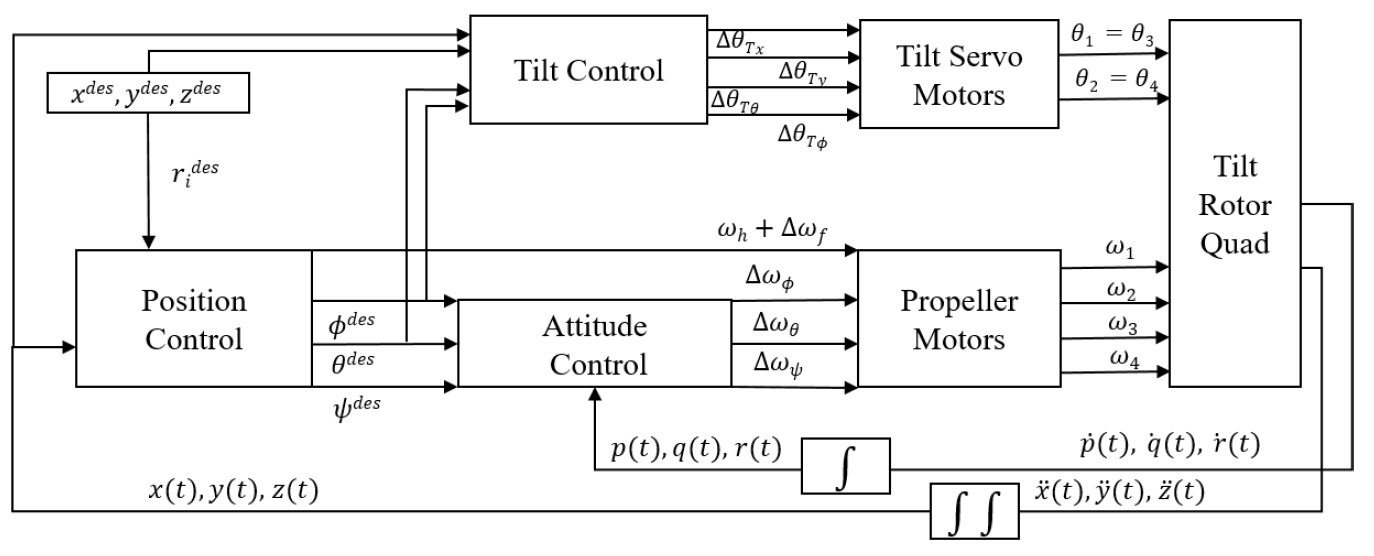
\includegraphics[width=.95\linewidth]{figures/control_arq.PNG}
        \caption{Control Architecture of Tilting-Rotor quadrotor \cite{kumar2017position}.}
        \label{fig:control_arq}
    \end{center}
\end{figure}

\section{Expected implementation route}
With the theory defined, it is possible to plan the implementation route that is expected to be followed during the development of the project, along which it is normal to find problems or inconsistencies that may require re-planning or redesign, issues that will be addressed in the implementation chapter \ref{impl}.\\

Initially, the following plan is expected to be followed:

\begin{enumerate}
    \item \textbf{CAD Model Development} It will consist of the design of a quadrotor with 2 degrees of freedom in its propellers (radial and tangential) that will serve as a simulation base for this project.
    
    \item \textbf{Integration of the model into CoppeliaSim} It includes all the procedures required to integrate the generated CAD design, the visual dynamics of the propellers, definition of its hierarchical structure and the coding of the scripts required for the implementation of the designed control.

    \item \textbf{Tuning gains and iterative experimentation} It consists of the tuning and experimentation cycle that allows the selection of the required gains to obtain an appropriate control for the required task.
\end{enumerate}

\chapter{Implementation}\label{impl}
This section of the report describes the critical points and decisions made throughout the implementation of the project, with special attention to turning points related to the implementation of the control and the tuning process.

\section{CAD Model Development}
The type of quadcopter chosen for this project is with standard design with propellers tilting in $S^2$ (i.e., both radially and tangentially) making it an over actuated system. The preliminary model is obtained from GRABCAD Community \cite{NicholasVonKlemperer}. 

\begin{figure}[H]
    \begin{center}
        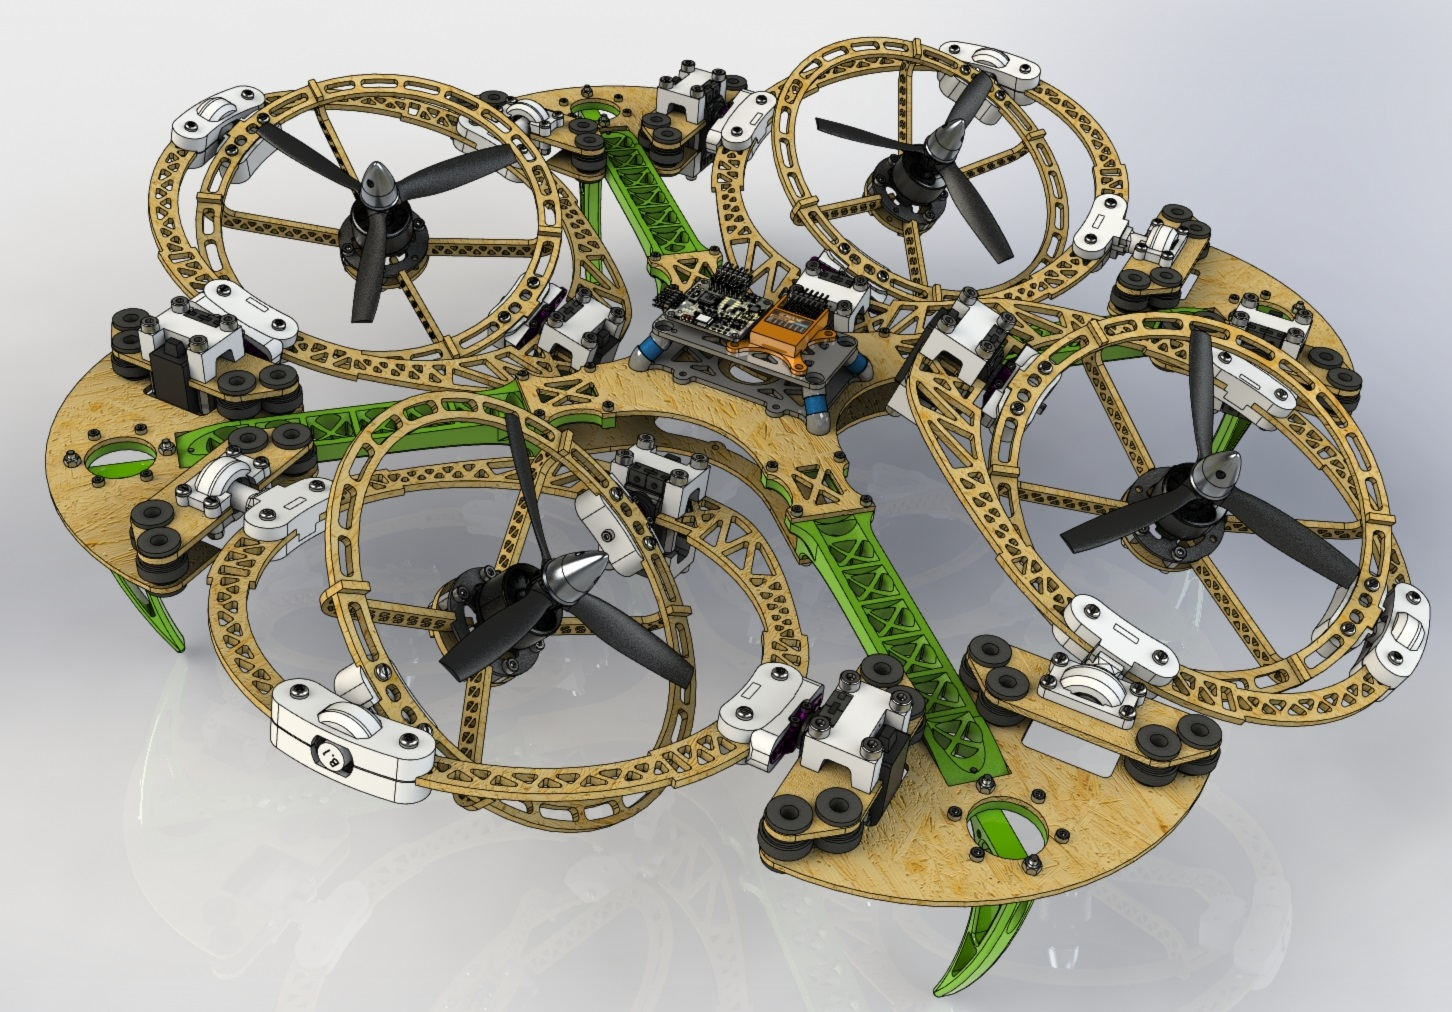
\includegraphics[width=.6\linewidth]{figures/DesignFull.JPG}
        \caption{3D model of Tilting-Rotor quadrotor.}
        \label{fig:3dmodel}
    \end{center}
\end{figure}

The rendered model is as shown in the figure \ref{fig:3dmodel}. As it can be seen in the figure, each propeller can be tilted radially and tangentially apart from the propeller rotation. The tilt angles are controlled by servo motors and fast enough to ignore the control loop.\\

The model obtained is set of all the parts in building the quadcopter. These parts are in "SLDPRT" format which can be edited using the SolidWorks software as shown in the figure \ref{fig:solidworksPart}. The parts are first properly assembled by assigning their respective mates which is either fixed or concentric mate. Finally the assembled model is obtained in "SLDASM" format. Note that all the propeller axis are facing upward to obtain proper coordinate frame. The assembly is done such a way that the body's z-axis faces upward and the x-axis towards the first propeller marking that as the forward motion. Similarly y-axis is towards the left propeller which is the standard format required for CoppeliaSim. 

\begin{figure}[H]
    \begin{center}
        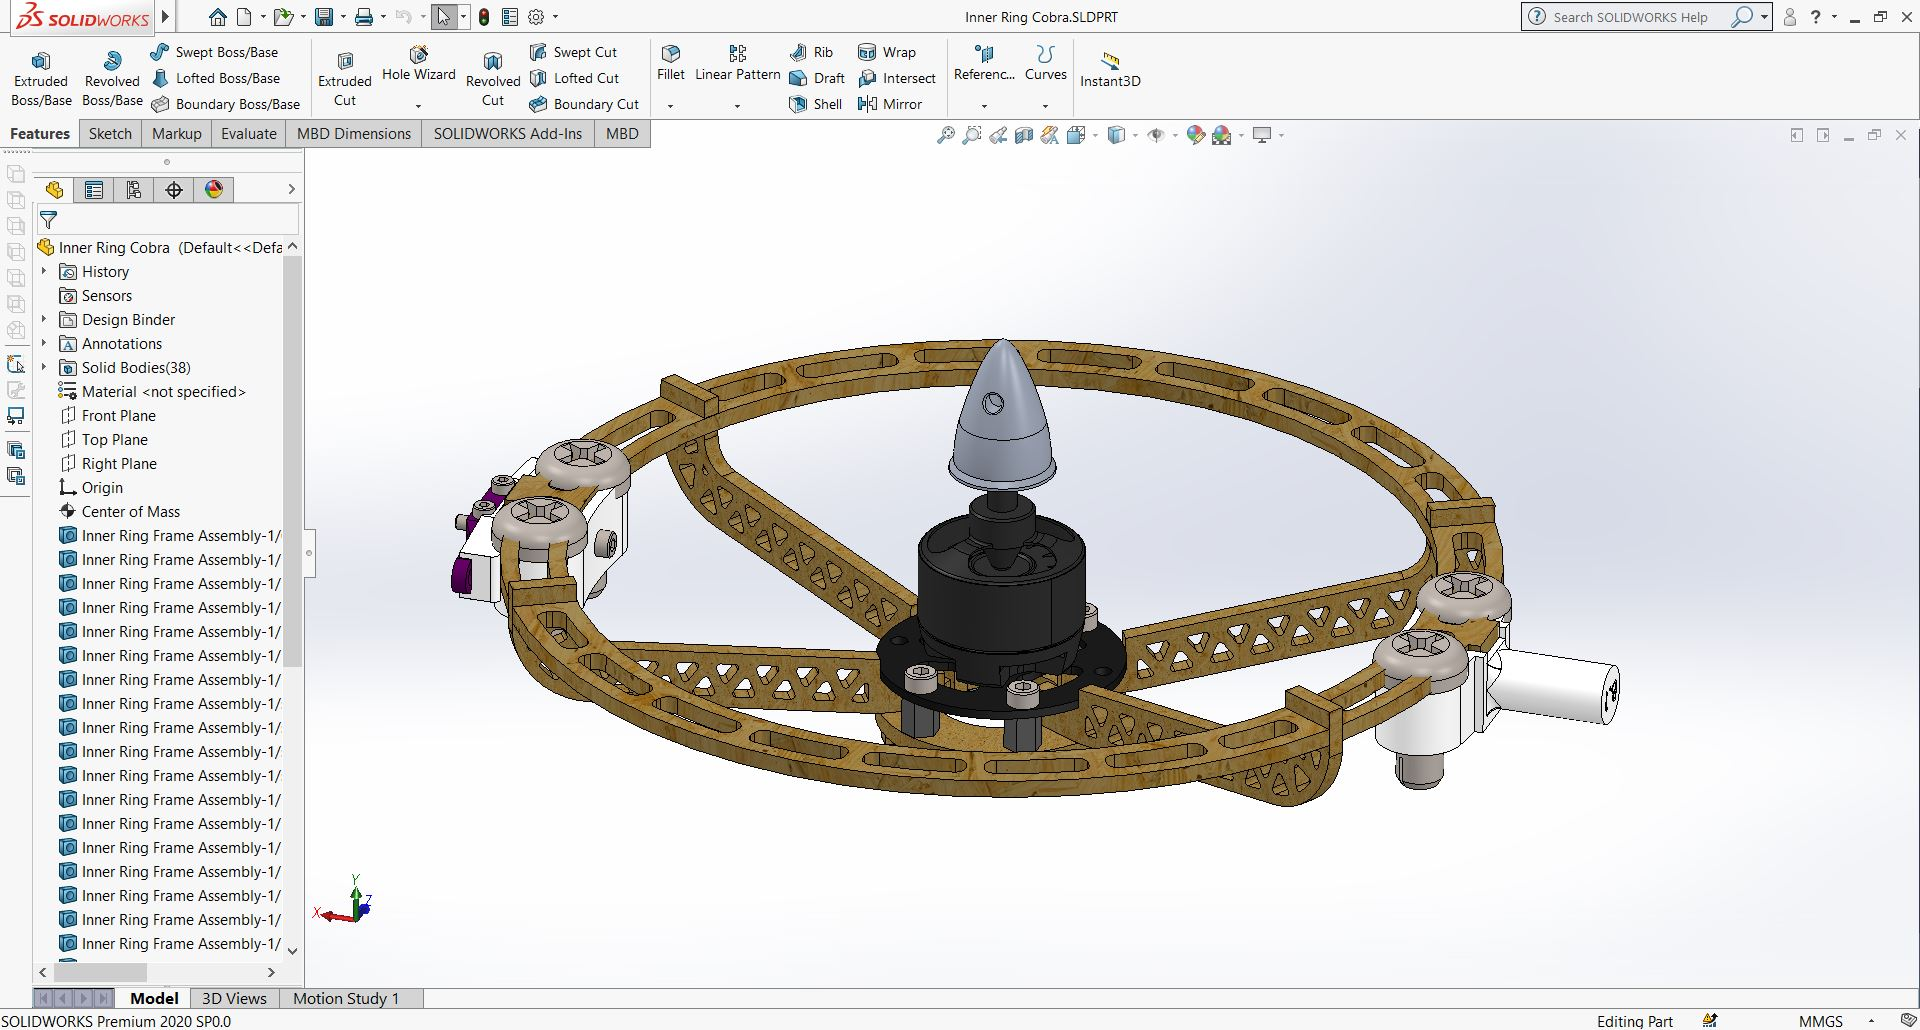
\includegraphics[width=.8\linewidth]{figures/individualAssem.JPG}
        \caption{Single propeller assembled in SolidWorks.}
        \label{fig:solidworksPart}
    \end{center}
\end{figure}

The last step is obtaining the right files which are compatible with CoppeliaSim. The assembled model in SolidWorks can be used to obtain the individual files in "STL" format along with their reference frame with respect to the the model's coordinate point. This will help in placing the parts in CoppeliaSim exactly where they belong.

\section{Integrating model into CoppeliaSim}
This is the most crucial step in the scene development as the model should be properly structured and simulation friendly. There are multiple steps which has to be followed that is explained in this section.

\subsection{Part grouping and assigning materials}
The SolidWorks generate large number of STL files (one for each part) and as a result, there are 160 files in total. Of course this is a huge set and relevant parts has to be grouped together to make the scene more simpler. This can be done by selecting multiple non-pure shapes and choosing grouping option available inside edit command as shown in the figure \ref{fig:merge}. This will generate a single multishape non-pure object. This is to be done to all the parts that has fixed mates and which does not move individually. Therefore the model will be reduced to only 13 multishape non-pure objects (1 body, 4 propellers, 4 radial tilt rings and 4 tangential tilt rings) that are the total links in the quadcopter. These objects can by assigned with different colors, texture and materials for better visualization.  

\begin{figure}[H]
    \begin{center}
        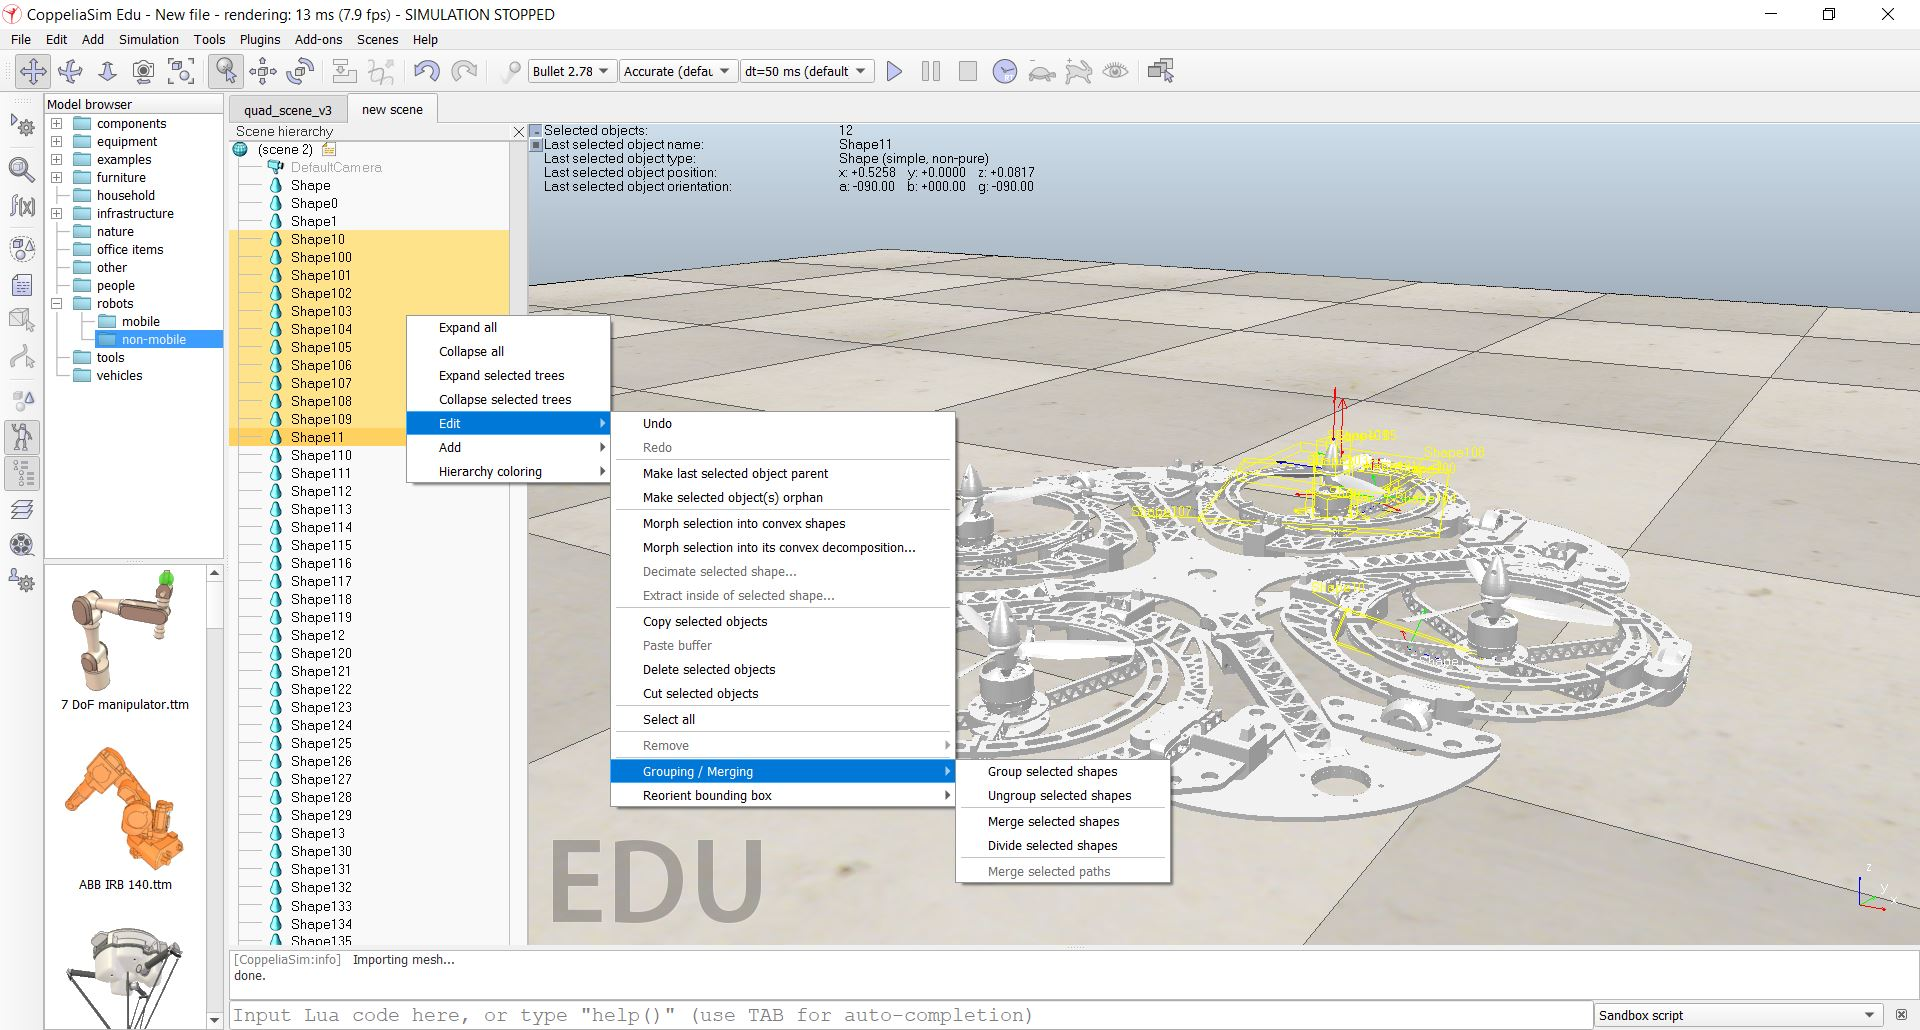
\includegraphics[width=.95\linewidth]{figures/merging_step.JPG}
        \caption{The figure shows the grouping of merging future for multiple non-pure shapes using CoppeliaSim.}
        \label{fig:merge}
    \end{center}
\end{figure}

\subsection{Develop pure shapes}
Since we will be performing dynamic simulation, the model should have respondable shapes. It is recommended to use pure shapes as they are more stable and faster. This is because of the large reduction in number of triangular meshes in the actual model. The total number of meshes for the entire model is in the range of hundred thousand as it is a very complex model whereas by generating pure shapes, this can be reduced to just hundreds. \\

\begin{figure}[H]
    \begin{center}
        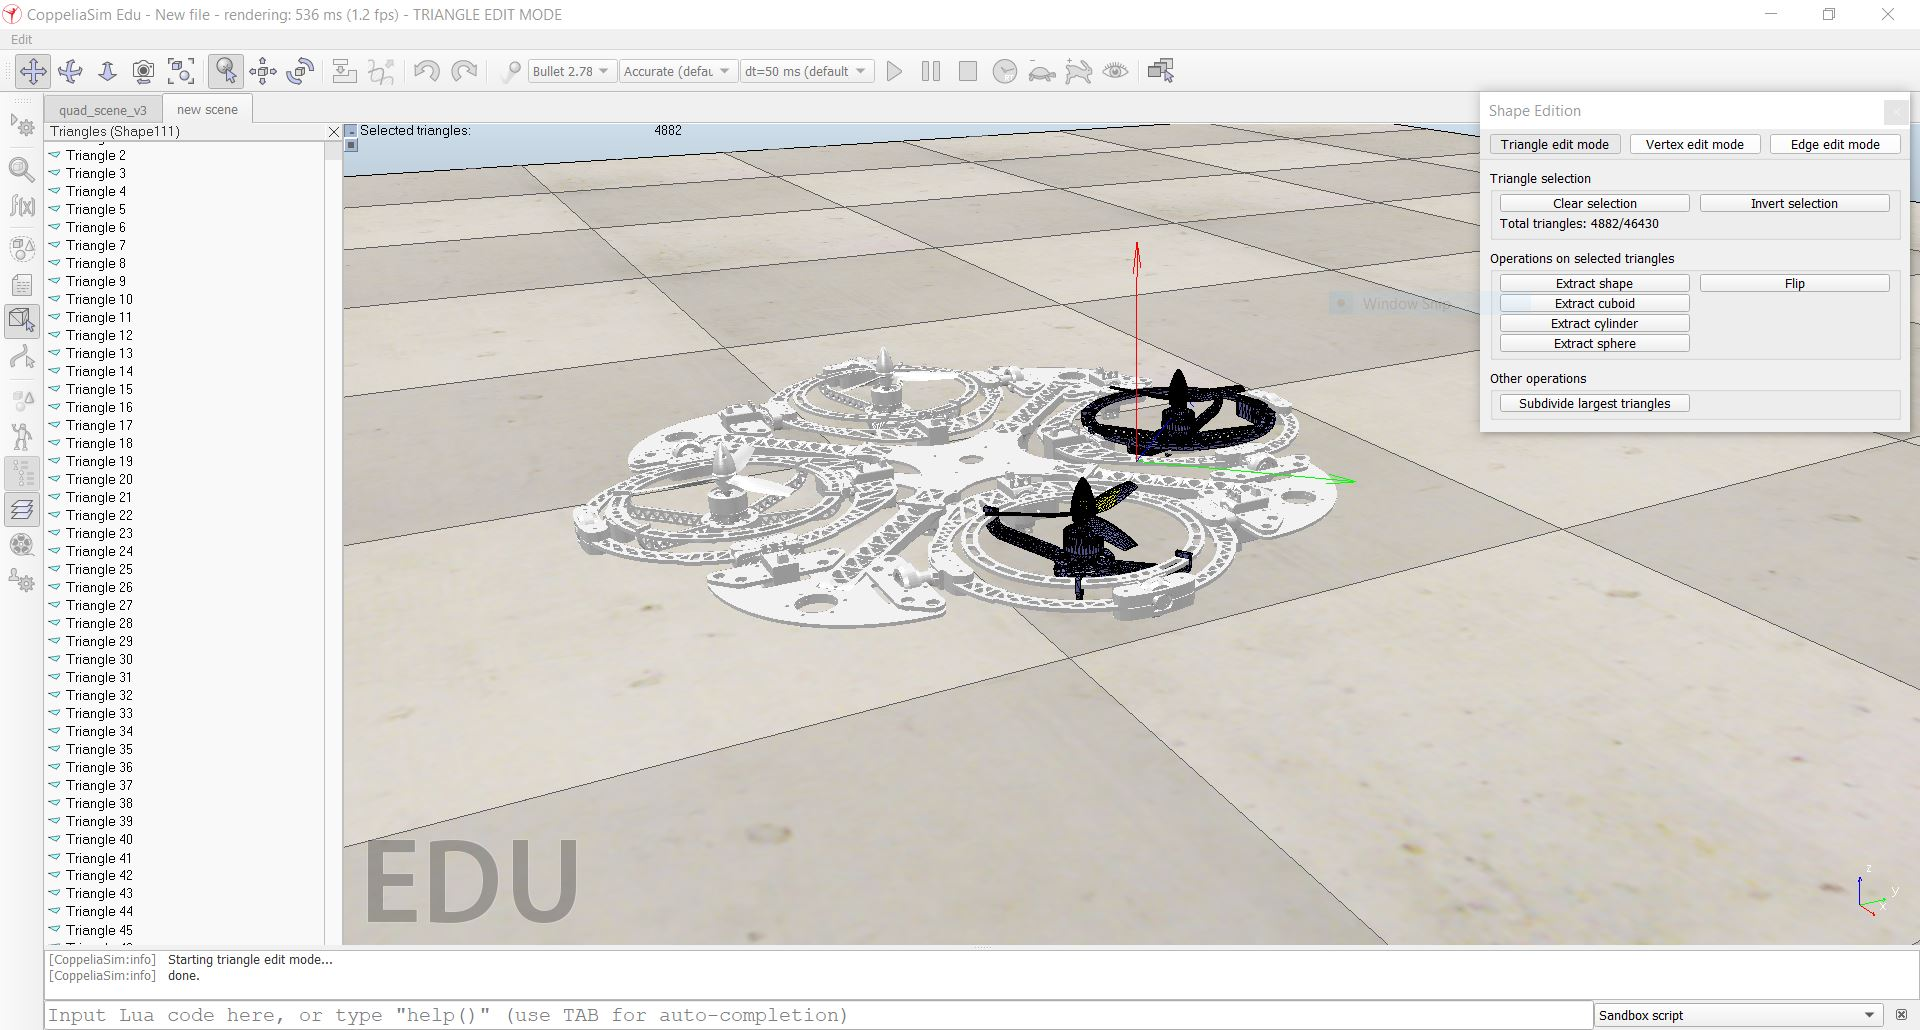
\includegraphics[width=.95\linewidth]{figures/extractShape.JPG}
        \caption{The figure shows the triangle edit mode available in CoppeliaSim.}
        \label{fig:extractShape}
    \end{center}
\end{figure}

This can be done by first merging all the shapes inside a single multishape non-pure object and entering into triangle edit model as shown in the figure \ref{fig:extractShape}. The relevant triangles are selected and then a shape of type cuboid, cylinder or sphere can be extracted from that. This will be a pure shape and it has to be done to all the links to finally obtain pure objects for each of them as shown in the figure \ref{fig:hiddenLayer}. Finally these a set of pure shapes are obtained which is moved to the hidden layer as these does not have to be visualised.

\begin{figure}[H]
    \begin{center}
        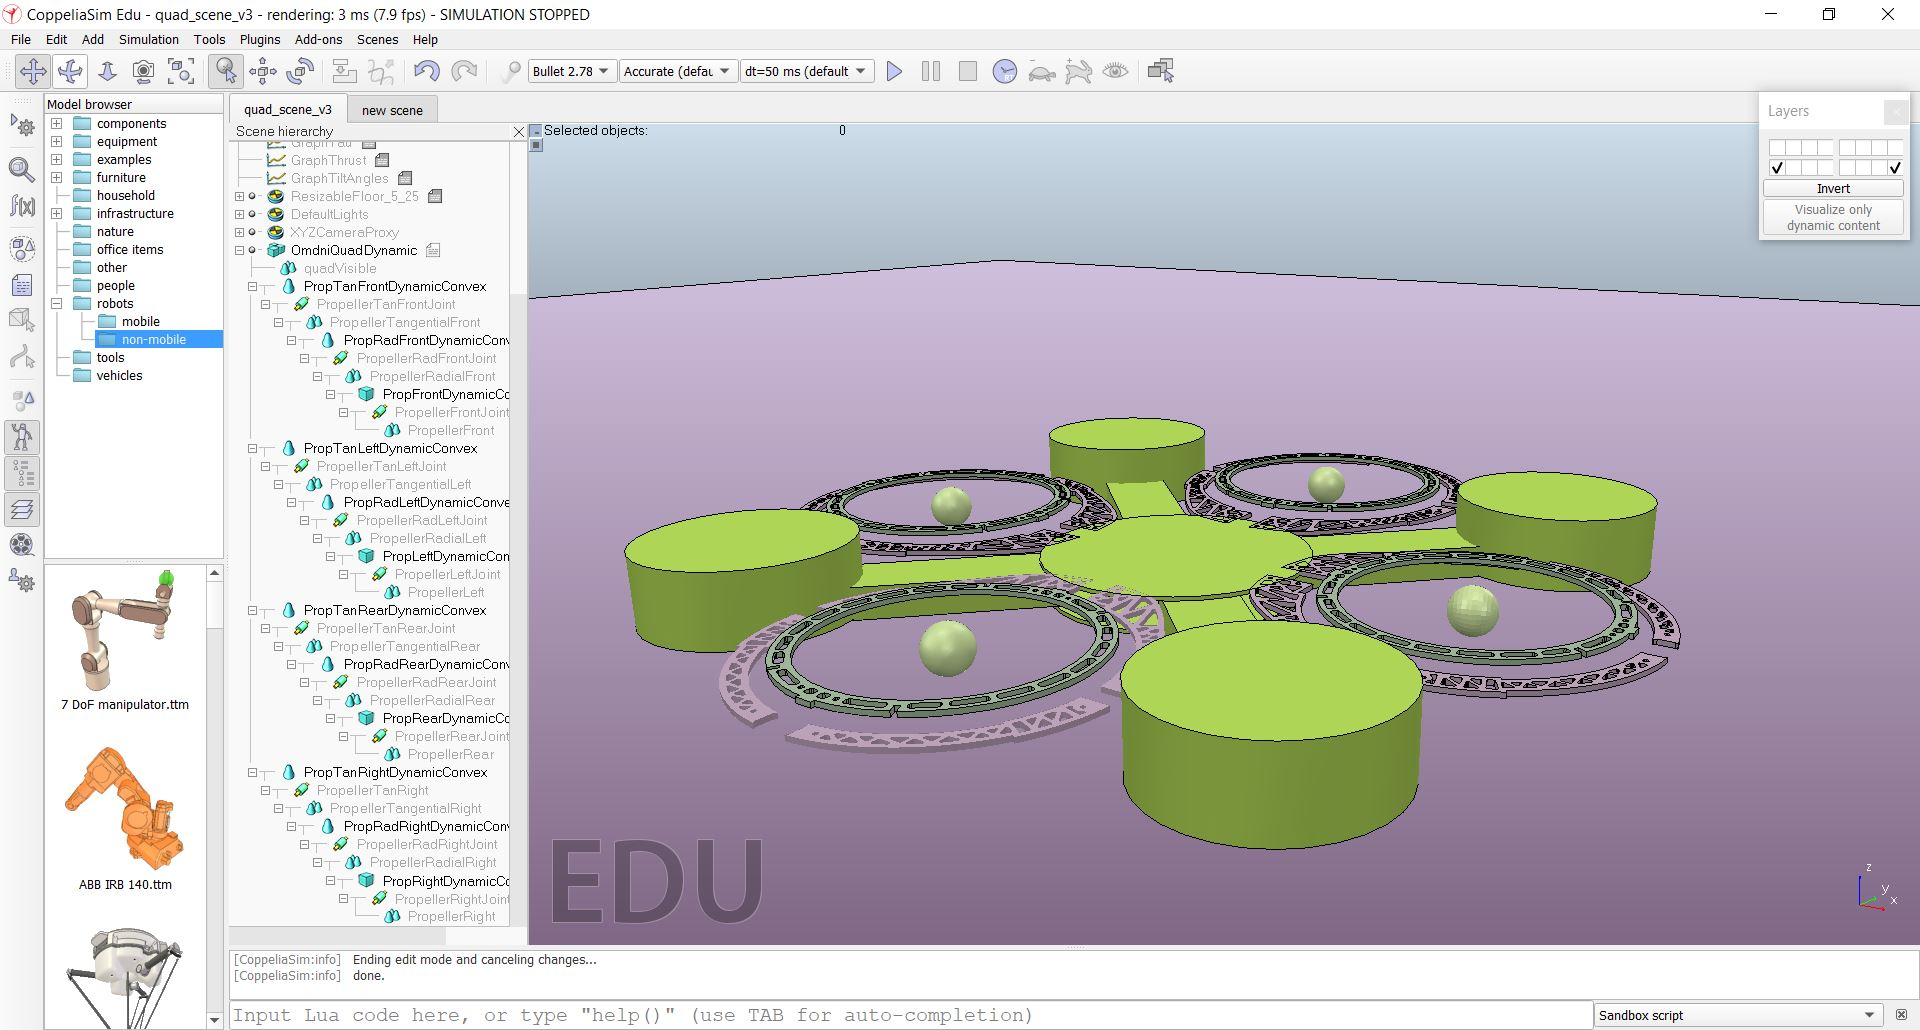
\includegraphics[width=.95\linewidth]{figures/hidden_layer.JPG}
        \caption{The figure shows the final hidden layer with all pure shapes}
        \label{fig:hiddenLayer}
    \end{center}
\end{figure}

\subsection{Adding joints}
The next crucial step is to generate joint objects. The joint objects as the name suggests provide a method to assign type of motion (revolute, prismatic or sperical) based on the requirement in the model. The main difficulty is to find the exact position and orientation for these joints. This can be done by carefully extracting pure shapes using triangle edit mode from the physical object's joint shaft. These pure objects are dealt as dummy objects which are used to assign position to the joint objects and later deleted. The final result from this step is as shown in the figure \ref{fig:joints}. 

\begin{figure}[H]
    \begin{center}
        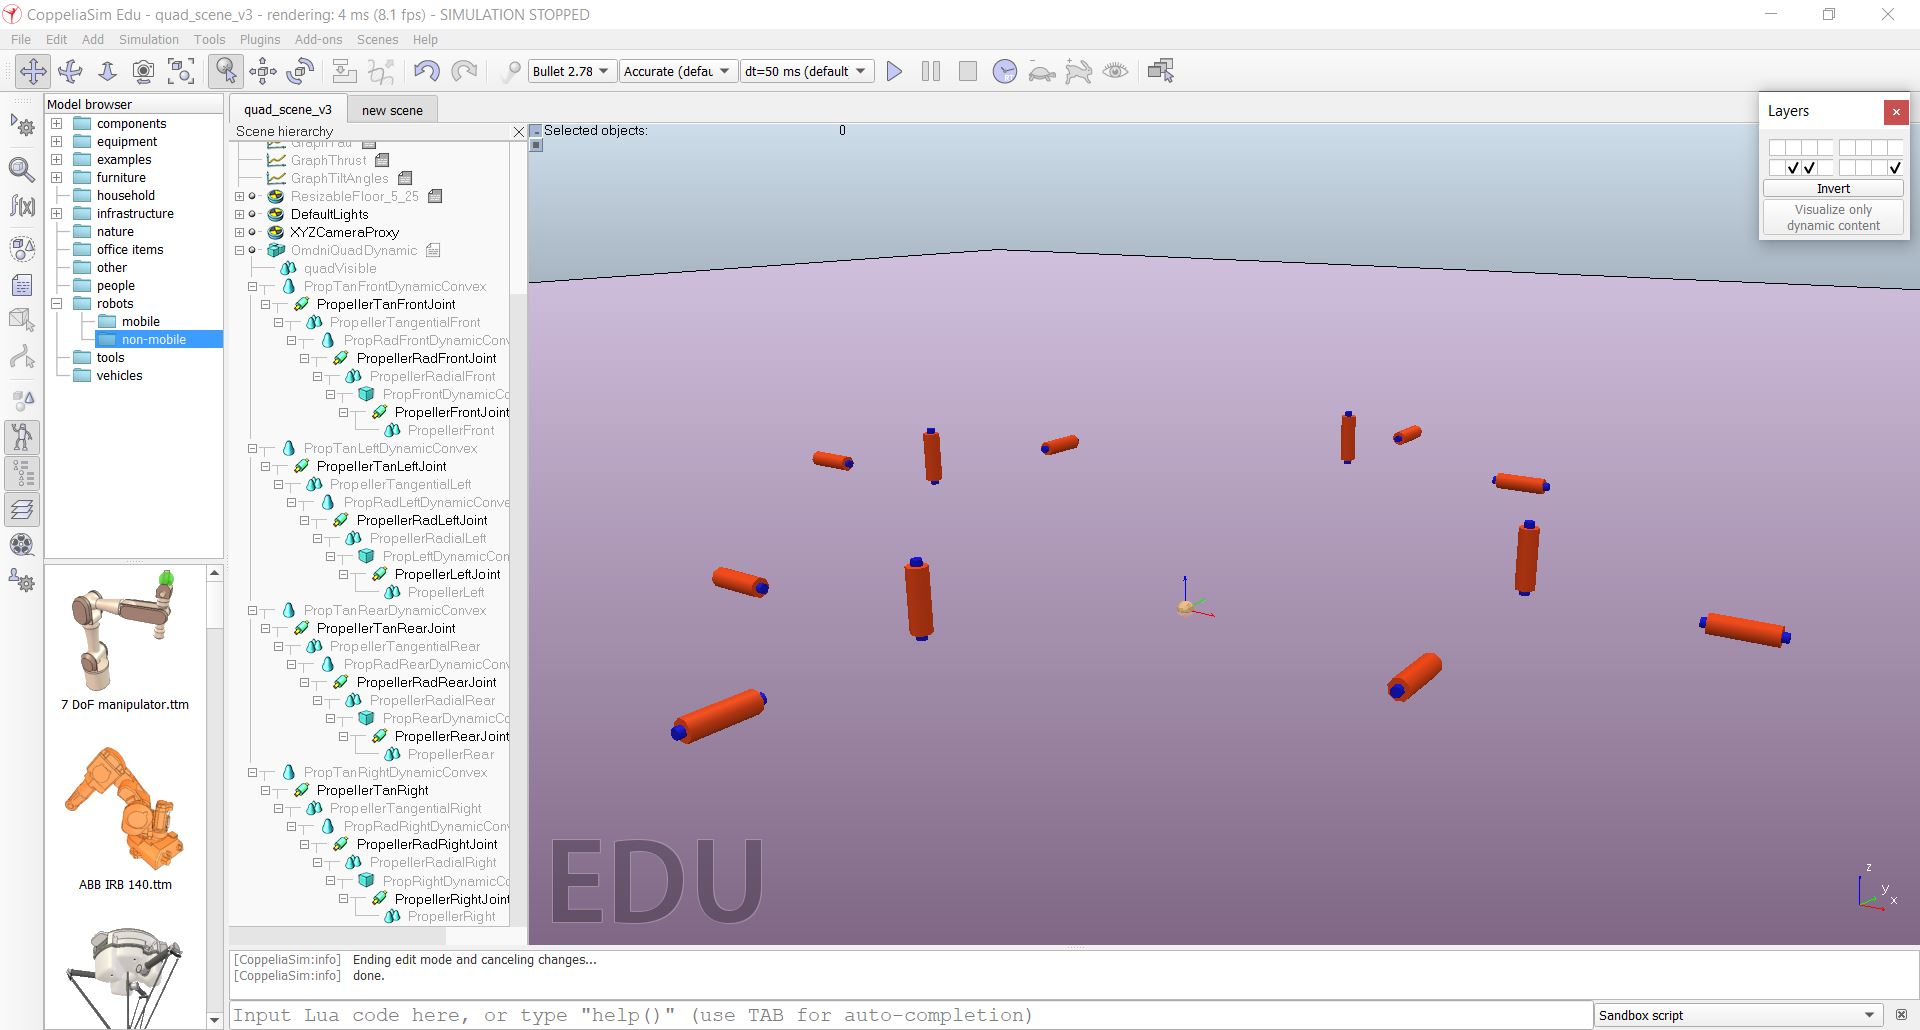
\includegraphics[width=.95\linewidth]{figures/joints.JPG}
        \caption{The figure shows the joints in space}
        \label{fig:joints}
    \end{center}
\end{figure}

\subsection{Developing parent-child structure}
Until now, all the objects required for the model are been developed and the next step is to setup the hierarchy. The structure has the base link which is the skeleton of the robot. All the pure parts which are relevant to the skeleton are grouped together and this is considered as the main parent object which contains all the other objects. The next object will be multishape non-pure object of the skeleton and all the tangential tilt rings as this is the link connected to the skeleton. \\

Next step is to add the revolute joints to their respective tangential tilt rings. Moving further the hierarchy has similar structure i.e., pure shape, then the joint and finally the non pure shape for all the links. The final hierarchy is as shown in the figure \ref{fig:heirarchy}.    

\begin{figure}[H]
    \begin{center}
        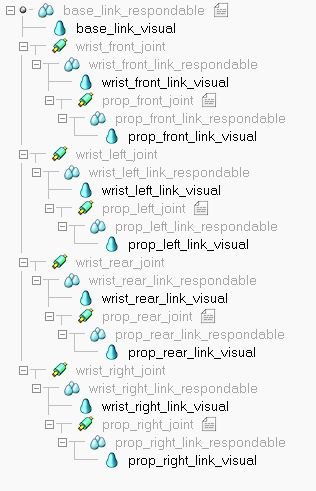
\includegraphics[width=.40\linewidth]{figures/heirarchyV2.JPG}
        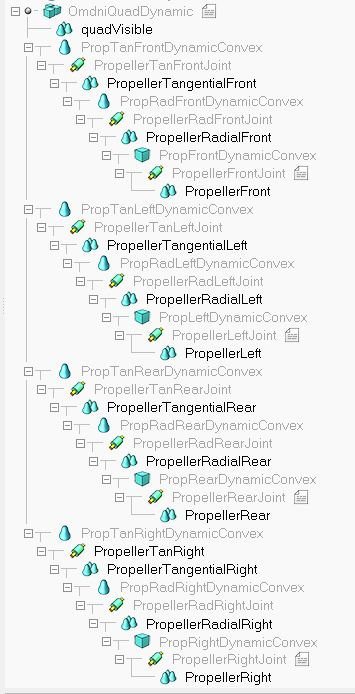
\includegraphics[width=.40\linewidth]{figures/heirarchyV3.JPG}
        \caption{The two versions of scene hierarchy. The left version has only radial tilt and non pure parts. The right version is $S^2$ type and has pure parts.}
        \label{fig:heirarchy}
    \end{center}
\end{figure}

\subsection{Develop Lua script}
The final step is to write the script to implement control design explained in the methodology chapter \ref{meth}. Since the simulation of air particle flow is very complex to design and requires large computation power, a simpler approach is followed in which the force and torque calculated from the equations are send to the skeleton of the quadcopter and propellers are simply rotated at a fixed speed for visualization purposes. However, the correct tilt angles are visualised as that is an important part of the project. \\

The main script where the attitude control is done is put in the first parent pure object. This is a non-threaded child script which runs individually as soon as the simulation is started. The script has mainly three functions which are sysCall\_init(), sysCall\_actuation(), and sysCall\_sensing(). All the global variables and object handlers are defined in the init function. The handlers are nothing but the references to the child objects on which the commands are sent/received. The actuation function deals in computing the control inputs and sending force and torques to the skeleton body along with tilt angles to the respective tilt joints. Finally, the sensing function is where all the feedback values required for control design is obtained.   

\section{Tuning gains and Iterative Experimentation}\label{tune}
The final step is to tune the gains of the attitude control implemented as explained in section \ref{control}. Since this is a fully actuated system with 6 control inputs, there are around 20 gains which is to be tuned to perform smooth attitude control. To make the task simpler, the approach that is followed is by independently tuning each control input by setting the others to zeros. This way, a somewhat smoother trajectory is obtained which is then fine tuned to behave smoothly.\\

One of the issues faced during the tuning phase was that the forces where applied only in z axis. This was forcing the model to move in only z axis even when there are forces acting on other directions. This was fixed by moving the reference frame on the robot by homogeneous transformation of the ground and the robot frame. Finally a simple attitude control is designed.   

\chapter{Experiments and Results}\label{expe}
The goal of the project is to develop an over actuated quad design as a CoppeliaSim scene. Based on the implementation discussed in previous section, the final scene of quadcopter with radial and tangential tilt is achieved. The final scene is shown in the figure \ref{fig:finalScene}.

\begin{figure}[H]
    \begin{center}
        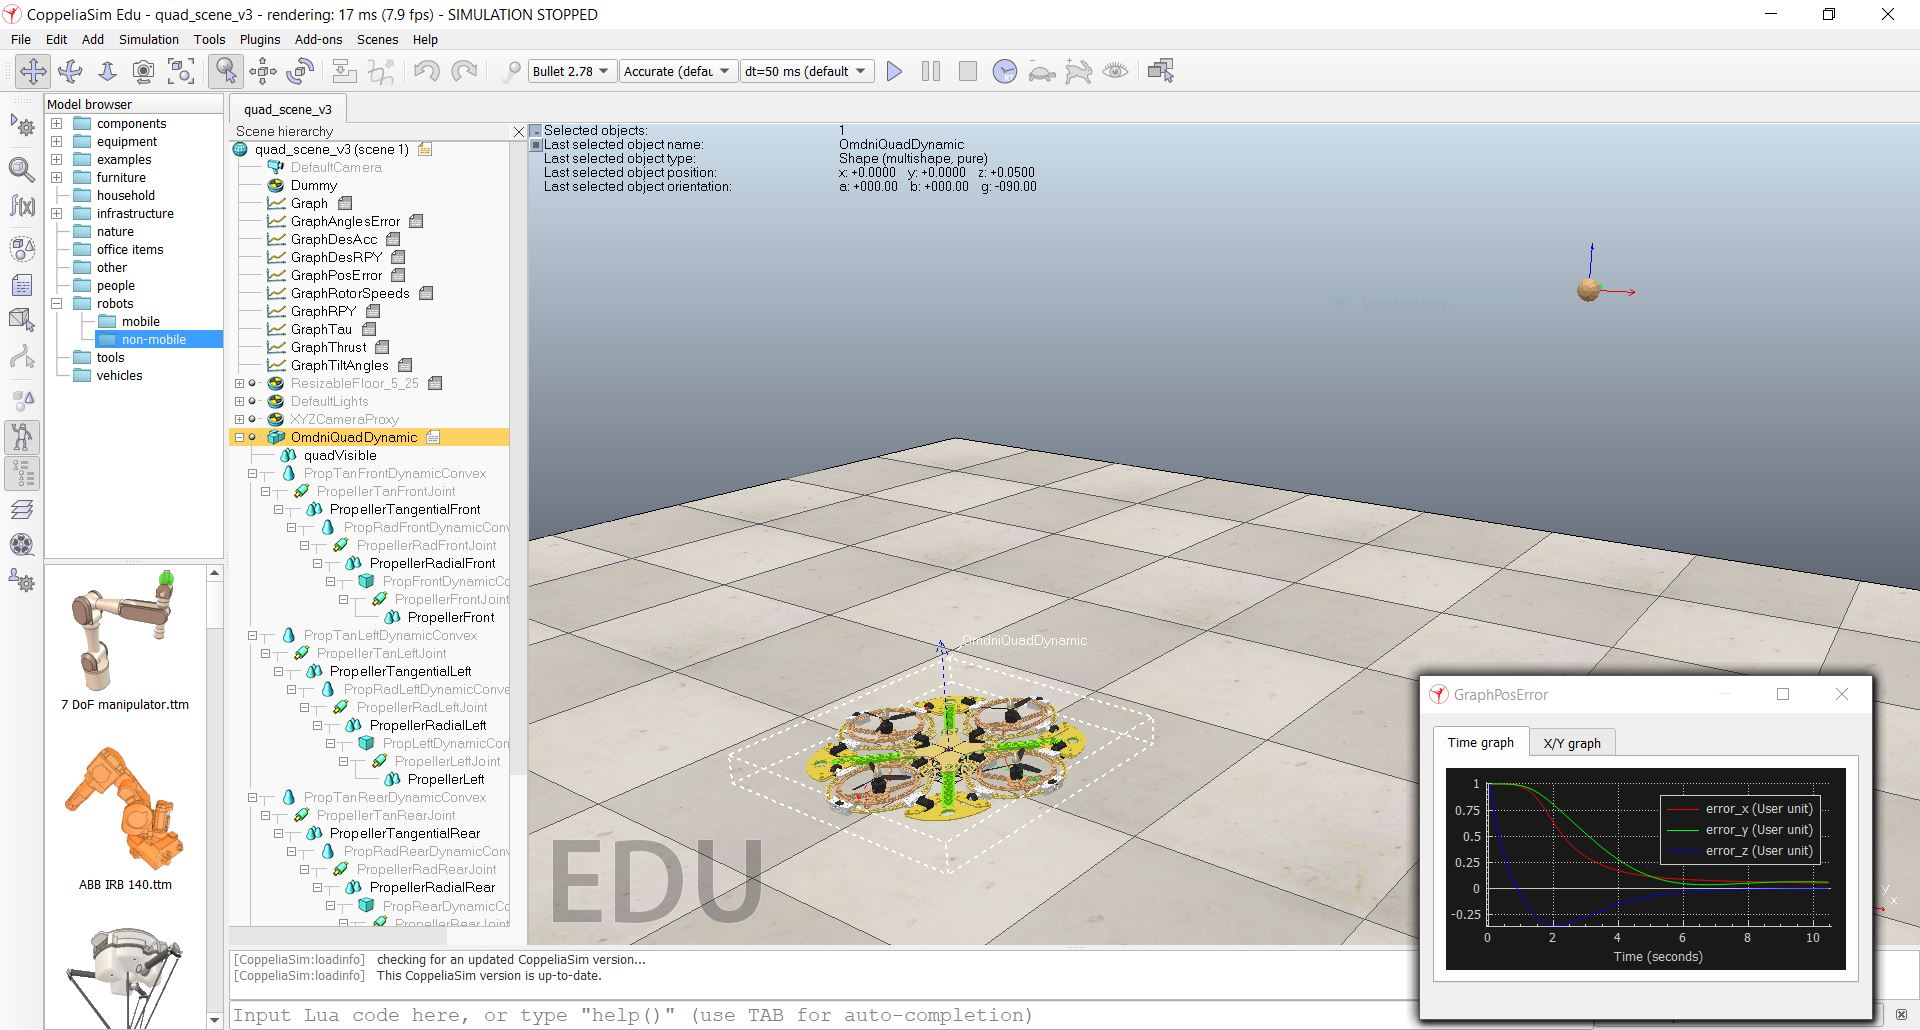
\includegraphics[width=.95\linewidth]{figures/finalScene.JPG}
        \caption{The figure shows the final CoppeliaSim scene with dummy object showing the desired position to be reached by attitude control.}
        \label{fig:finalScene}
    \end{center}
\end{figure}

To prove the model, a simple attitude control is implemented to reached a desired position and orientation and hover at that point. The gains were tuned as mentioned in section \ref{tune}. The final result of attitude control is shown in the figure \ref{fig:attitudeControl}. The blue line in the scene shows the trajectory followed by the robot during the simulation. \\

\begin{figure}[H]
    \begin{center}
        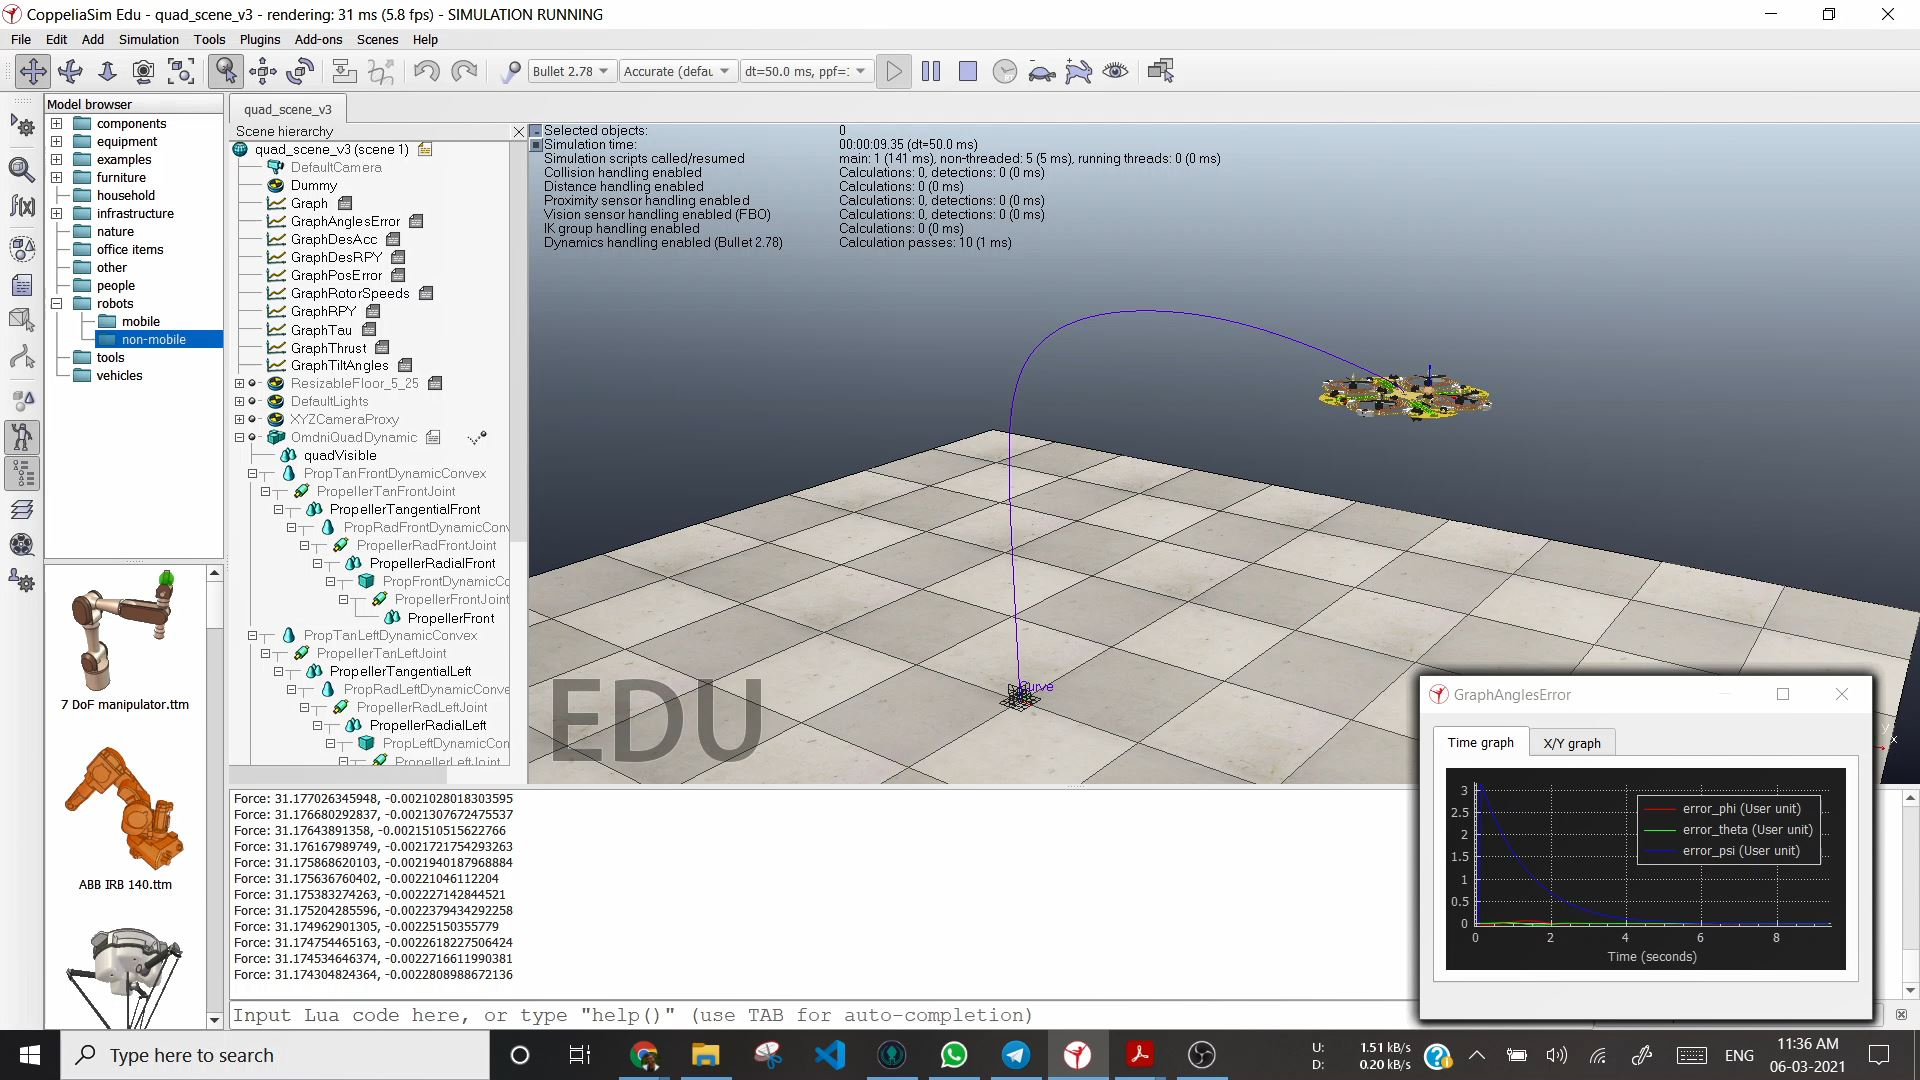
\includegraphics[width=.95\linewidth]{figures/goalReach.JPG}
        \caption{The figure shows the attitude control for a desired position and orientation with blue line showing the path followed.}
        \label{fig:attitudeControl}
    \end{center}
\end{figure}

Although the model is designed as a quadcopter with both radial and tangential tilt capabilities. The attitude control is developed with only radial tilt. This can be further improved with various other control types by taking the model as an over actuated system as it is. However, the goal of building a scene is successfully achieved. 

\chapter{Conclusion}\label{conclu}
In accordance with the scope proposed for this project, the objectives defined were fully met by designing an over-actuated UAV model, suitable for the implementation and testing of control models in a simulated environment. This model has the degrees of freedom required so that its propellers can direct the thrust vector in $S^2$ and is fully integrated with CoppeliaSim, thus being a ready platform for future developments and projects.\\

Specifically, the mathematical requirements that support the conversion of an over-actuated UAV to a fully-activated one were also investigated to simplify the implementation of the control by disabling tangential tilt and mirroring the radial tilt in opposite propellers, a theory that was effectively implemented in the LUA script and verified with the graphical behavior of the UAV model in space, which effectively shows the drone movement and the propellers inclination.\\

From this point on, the tuning and experimentation cycle was successfully executed to find the gains associated with the controller to ensure proper convergence to a UAV pose (position and orientation).

\bibliographystyle{plain}
\bibliography{refs.bib}
\end{document}